% !TEX TS-program = pdflatex
% !TEX encoding = UTF-8 Unicode

% This is a simple template for a LaTeX document using the "article" class.
% See "book", "report", "letter" for other types of document.

\documentclass[11pt]{article} % use larger type; default would be 10pt

\usepackage[utf8]{inputenc} % set input encoding (not needed with XeLaTeX)

%%% Examples of Article customizations
% These packages are optional, depending whether you want the features they provide.
% See the LaTeX Companion or other references for full information.

%%% PAGE DIMENSIONS
\usepackage{geometry} % to change the page dimensions
\geometry{a4paper} % or letterpaper (US) or a5paper or....
\geometry{margin=1in} % for example, change the margins to 2 inches all round
% \geometry{landscape} % set up the page for landscape
%   read geometry.pdf for detailed page layout information

\usepackage{graphicx} % support the \includegraphics command and options

% \usepackage[parfill]{parskip} % Activate to begin paragraphs with an empty line rather than an indent
\usepackage{amssymb}
\usepackage{amsmath}
%%% PACKAGES
\usepackage{booktabs} % for much better looking tables
\usepackage{array} % for better arrays (eg matrices) in maths
\usepackage{paralist} % very flexible & customisable lists (eg. enumerate/itemize, etc.)
\usepackage{verbatim} % adds environment for commenting out blocks of text & for better verbatim
\usepackage{subfig} % make it possible to include more than one captioned figure/table in a single float
% These packages are all incorporated in the memoir class to one degree or another...

%%% HEADERS & FOOTERS
\usepackage{fancyhdr} % This should be set AFTER setting up the page geometry
\pagestyle{fancy} % options: empty , plain , fancy
\renewcommand{\headrulewidth}{0pt} % customise the layout...
\lhead{}\chead{}\rhead{}
\lfoot{}\cfoot{\thepage}\rfoot{}

%%% SECTION TITLE APPEARANCE
\usepackage{sectsty}
\allsectionsfont{\sffamily\mdseries\upshape} % (See the fntguide.pdf for font help)
% (This matches ConTeXt defaults)

%%% ToC (table of contents) APPEARANCE
\usepackage[nottoc,notlof,notlot]{tocbibind} % Put the bibliography in the ToC
\usepackage[titles,subfigure]{tocloft} % Alter the style of the Table of Contents
\usepackage{bbm}
\usepackage{endnotes}

\renewcommand{\cftsecfont}{\rmfamily\mdseries\upshape}
\renewcommand{\cftsecpagefont}{\rmfamily\mdseries\upshape} % No bold!
\DeclareMathOperator*{\argmax}{arg\,max}
\DeclareMathOperator*{\argmin}{arg\,min}

\usepackage{graphicx}
\graphicspath{ {./pings/} }

\newcount\colveccount
\newcommand*\colvec[1]{
        \global\colveccount#1
        \begin{pmatrix}
        \colvecnext
}
\def\colvecnext#1{
        #1
        \global\advance\colveccount-1
        \ifnum\colveccount>0
                \\
                \expandafter\colvecnext
        \else
                \end{pmatrix}
        \fi
}

\newcommand{\norm}[1]{\left\lVert#1\right\rVert}

\title{Econometrics HW6}
\author{Michael B. Nattinger\footnote{I worked on this assignment with my study group: Alex von Hafften, Andrew Smith, and Ryan Mather. I have also discussed problem(s) with Emily Case, Sarah Bass, Katherine Kwok, and Danny Edgel.}}

\begin{document}
\maketitle

\section{Question 27.1}
\begin{align*} % use theorem 5.8.2 <- wrong, use 5.8.4
m(X) = E[Y|X] &= E[\max\{ X'\beta + e,0\}|X] \\
&= E[(X'\beta+e) 1\{X'\beta+e >0 \}|X]\\
&= X'\beta\left(1-\Phi\left(\frac{ -X'\beta}{\sigma}\right)\right) + \sigma \phi\left(\frac{-X'\beta}{\sigma}\right) \\
&= X'\beta\Phi\left(\frac{ X'\beta}{\sigma}\right)+ \sigma \phi\left(\frac{X'\beta}{\sigma}\right).
\end{align*}

\begin{align*} % use theorem 5.7.6 <- wrong, use 5.8.6
m^{\#}(X) = E[Y^{\#}|X] &= E[X'\beta+e|X'\beta+e>0]\\
&= X'\beta + \sigma\lambda\left(\frac{X'\beta}{\sigma}\right).
\end{align*}
\section{Question 27.2}
OLS is not consistent for $\beta$. $\beta $ will be biased towards zero as the best-fit line through $Y^{*}$ will be flatter than it would have been through $Y$.
\section{Question 27.3}
\subsection{Part A}
Yes, $\hat{\beta}$ will be consistent for $\beta$, which we can show. Let $n$ be the number of observations which satisfy the condition that $X_1>0$, and let $X,Y$ be the corresponding data which satisfies the condition. 
\begin{align*}
\hat{\beta} &= \left( \frac{1}{n} \sum_{i=1}^n X_i X_i' \right)^{-1} \left( \frac{1}{n} \sum_{i=1}^n X_i Y_i\right) \\
&= \beta + \left( \frac{1}{n} \sum_{i=1}^n X_i X_i' \right)^{-1} \left( \frac{1}{n} \sum_{i=1}^n X_i e_i\right) \\
&\rightarrow_p \beta + E[X_iX_i'|X_{1i}>0]^{-1}E[X_ie_i|X_{1i}>0]\\
&= \beta.
\end{align*}
\subsection{Part B}
No, this is not consistent. The mathematical argument is the same but in the probability limit the conditioning on the error is different and induces bias:
\begin{align*}
\hat{\beta} &\rightarrow_p \beta + E[X_iX_i'|Y_{i}>0]^{-1}E[X_ie_i|Y_{i}>0]\\
&= \beta +  E[X_iX_i'|X_{i}\beta +e_i>0]^{-1}E[X_ie_i|X_{i}\beta +e_i>0] \\
& \neq \beta.
\end{align*}
This does not equal $\beta$ in the probability limit because $E[X_ie_i|X_{i}\beta +e_i>0] \neq 0$ in general.
\section{Question 27.4}
The NLLS identification would be the sum of squared errors of the conditional probability distribution given a parameterization and the $Y$ data:
\begin{align*}
(\hat{\beta},\hat{\sigma}) &= \argmin_{\beta,\sigma} \sum_{i=1}^n \left(Y_i -X_i'\beta \Phi\left( \frac{X_i'\beta}{\sigma} \right) - \sigma \phi\left( \frac{X_i'\beta}{\sigma} \right) \right)^2
\end{align*}
\section{Question 27.8}
\begin{align*}
E[Y|X,Z,S=1] &= X'\beta + E[e|X,Z,S=1] \\
&= X'\beta + E[e|u>-Z'\gamma] \\
&= X'\beta + \rho_{2,1} E[u|u>-Z'\gamma]\\
&=X'\beta + \rho_{2,1}\lambda(Z'\gamma).
\end{align*}
\section{Question 27.9}
Regression results (point estimates) for the various parts of the question follow.

\begin{center}
\begin{tabular}{ll}
& beta \\ 
\hline 
education & 0.14431 \\ 
experience & 0.042633 \\ 
experience\^{}2/100 & -0.095056 \\ 
constant & 0.53089 \\ 
\hline 
\end{tabular}
\end{center}

Note that tinkind was originally negative over 10 \% of the time and therefore was not originally properly censored,  so I set any negative values of tinkind to 0. After this change, our results for part B are that 22.46\% of the observations are censored.  This is sufficiently high to expect censoring bias to be a problem in this example.

Interpreting the differences in results, we first note that the coefficients are all relatively similar. Next, note that the magnitudes of the coefficients are almost exactly the same for inc and Dinc, but the sign is different - this is because ind and Dinc are really similar series, with Dinc just being inc shifted to the left, except for the individuals who were already at 0.

Next, note that the CLAD and Tobit regressions yield very similar results. This is because these are unbiased estimates of very similar concepts. The two OLS estimates yield different results because they are biased towards zero.

Below are Matlab codes for the regressions. Note that I had to write code to estimate the CLAD regression, which I have included, as I could not find a pre-written CLAD routine online.

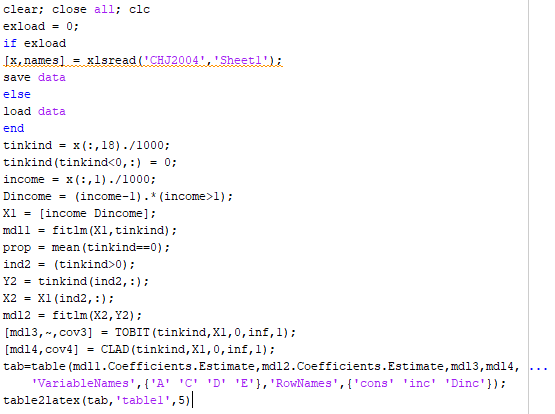
\includegraphics{p1}

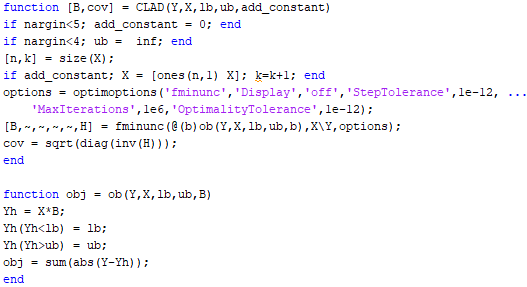
\includegraphics{p2}

\section{Question 28.12}
\begin{center}
\begin{tabular}{ll}
& results \\ 
\hline 
R\^{}2 & 0.38932 \\ 
SSE & 82.505 \\ 
\hline 
\end{tabular}
\end{center}

Above we can see the AIC, BIC of all of the models. The models we should choose should have the lowest AIC, BIC. The model with the lowest AIC is model (5), followed somewhat closely by model (8). The model with the lowest BIC is model (2), followed closely by model (5). My preferred choice would be model (5) as it performs well under both the AIC and BIC criterion, so it can robustly be considered a good choice in a wide variety of contexts.

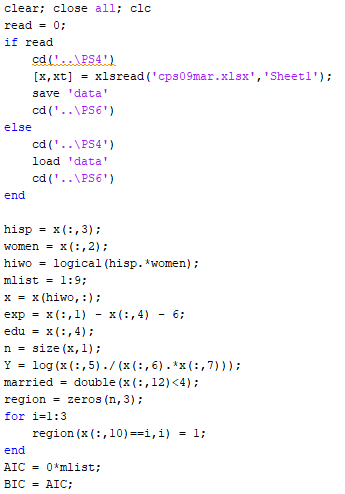
\includegraphics{p3}

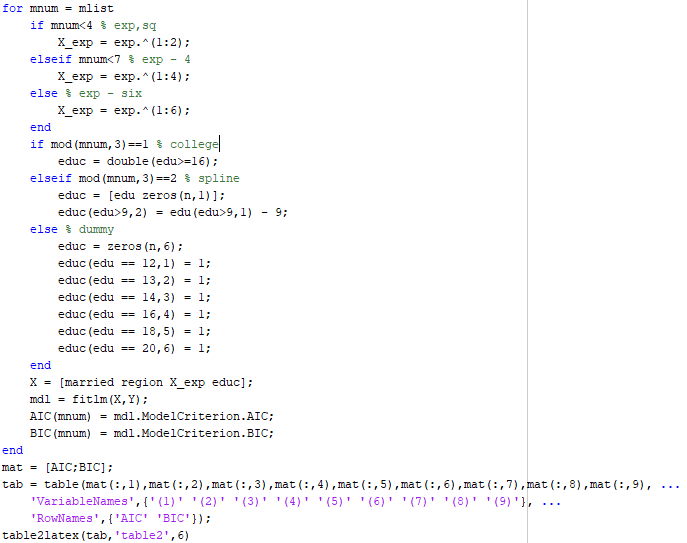
\includegraphics{p4}
\end{document}
